\documentclass[11pt]{article}

\usepackage[margin=1in]{geometry}
\usepackage[T1]{fontenc}
\usepackage[utf8]{inputenc}
\usepackage{lmodern}
\usepackage{microtype}
\usepackage{amsmath,amssymb}
\usepackage{booktabs}
\usepackage{array}
\usepackage{multirow}
\usepackage{graphicx}
\usepackage{xcolor}
\usepackage{hyperref}
\usepackage[nameinlink,noabbrev]{cleveref}

\hypersetup{
  colorlinks=true,
  linkcolor=blue!50!black,
  citecolor=blue!50!black,
  urlcolor=blue!50!black
}

\title{Localized Additive Composition of Persona and Task\\Near Answer Formation in Instruction-Tuned Language Models}
\author{Anonymous Submission}
\date{}

\begin{document}
\maketitle

\begin{abstract}
Role prompts of the form \emph{``As X, do Y''} are widely used, but the online computation that combines persona information $X$ and task information $Y$ is not well characterized. We study this question with a residual-stream $2\times2$ decomposition. For each persona-task pair, we compare baseline-baseline, persona-only, task-only, and persona-plus-task prompts, and define a pure persona effect $\Delta_X$, a pure task effect $\Delta_Y$, and an interaction term $\mathrm{Inter} = \Delta_{XY} - \Delta_X - \Delta_Y$. The central claim of the paper is that persona-task composition is approximately additive in a localized residual-stream region near answer formation, with explicit limits on what that local additivity does and does not imply.

The additive regime is \emph{localized but not point-like}: it spans the last prompt position $p_{\text{last}}$ and the first generated-token positions $g_1$ and $g_2$. On Gemma-2-2B-IT, additive substitution remains low-KL at all three positions in an early/mid-depth layer band, with median KL at $g_1$ of $0.049$ at layer 14 and at $g_2$ of $0.060$ at layer 14 on a 4-persona $\times$ 3-task grid. The same qualitative position-localized pattern recurs on Qwen-2.5-1.5B-Instruct and Qwen-2.5-3B-Instruct. Broadening prompt coverage to 8 long-form personas and 6 tasks (48 cells) leaves the localized additive regime intact: on Gemma-2-2B-IT median KL is $0.229$ at $p_{\text{last}}$, $0.056$ at $g_1$, and $0.056$ at $g_2$ at layer 14; on Qwen-2.5-1.5B-Instruct, the corresponding early-layer medians are $0.030$, $0.018$, and $0.014$.

Distributional similarity is not the same as behavioral correctness, so we complement the KL evidence with a behavioral-marker test: across 8 long personas $\times$ 3 review tasks, we score whether persona-specific markers (e.g., ``SPOF'' for the engineer persona, ``differential'' for the doctor persona) appear in the 80-token greedy continuation. Additive substitution at $p_{\text{last}}$, layer~14 recovers persona markers in 14 of 24 cells (58.3\%), close to the clean ceiling of 16 of 24 (66.7\%) and far above the bare-prompt floor of 1 of 24 (4.2\%) where the persona text is removed from the prompt.

We also retain an important negative result. Even when local additive substitution predicts next-step behavior well, substituting residuals into a baseline host prompt does not replace the information carried by persona text in context: on an 8-persona $\times$ 3-task long-persona setting, host-to-target median KL is $3.05$, cached single-site substitution reduces it only to $2.84$, and wider multi-layer substitution does not materially improve it. The clean conclusion is therefore not that role prompts are ``just vectors,'' but that persona-task composition is approximately additive in a localized residual-stream region near answer formation, while full prompt functionality remains distributed across the prompt and KV cache.
\end{abstract}

\section{Introduction}

Prompts of the form \emph{``As Warren Buffett, give advice''} or \emph{``As a senior software engineer, review this design''} are now routine. They are also mechanistically ambiguous. A model must combine persona information $X$ with task information $Y$ and produce behavior that reflects both. The central question of this paper is:

\begin{quote}
\textbf{How does an instruction-tuned language model combine persona information and task information in the residual stream near answer formation?}
\end{quote}

The most direct way to study this question is to avoid assuming in advance that the right object is a neuron, a head, or a circuit fragment. Instead, we start with the residual stream and ask whether persona and task contributions can be decomposed, and if so, where that decomposition is causally useful.

The residual-stream $2\times2$ decomposition gives a natural way to pose that question. For each persona-task pair, compare four prompts: baseline-baseline ($BB$), persona-only ($XB$), task-only ($BY$), and persona-plus-task ($XY$). At a fixed layer and position, define
\begin{align}
\Delta_X &= h_{XB} - h_{BB}, \\
\Delta_Y &= h_{BY} - h_{BB}, \\
\Delta_{XY} &= h_{XY} - h_{BB}, \\
\mathrm{Inter} &= \Delta_{XY} - \Delta_X - \Delta_Y.
\end{align}
The empirical question becomes concrete: is $\Delta_{XY}$ directionally aligned with $\Delta_X + \Delta_Y$? Are $\Delta_X$ and $\Delta_Y$ separated enough to be meaningful components? When we substitute $h_{BB} + \Delta_X + \Delta_Y$ for the clean $XY$ residual, does downstream behavior stay close to clean?

We do \emph{not} attempt a full-sequence mechanism. Instead, we ask whether the additive regime is localized to a small region near answer formation, whether that regime survives broader prompt coverage, and what explicit boundary conditions limit its interpretation.

The answer is a scoped positive. We find a localized additive regime spanning $p_{\text{last}}$ and the first two generated-token positions $g_1$ and $g_2$, strongest in early/mid layers and degrading later. We then show that the same qualitative pattern survives a much broader grid of long-form personas and diverse tasks, and recurs across Gemma and Qwen families. Finally, we show that this local additive structure does \emph{not} license a stronger claim that a persona prompt can be replaced by a single residual vector: host-prompt injection remains substantially short of the clean long-persona target. The resulting paper is deliberately narrower than a full mechanistic anatomy, but stronger for that reason.

\paragraph{Contributions.}
This paper makes five claims:
\begin{enumerate}
    \item A residual-stream $2\times2$ decomposition is a useful mechanistic abstraction for role prompts.
    \item The additive approximation is causally strong in a \emph{localized region} near answer formation, spanning $p_{\text{last}}$, $g_1$, and $g_2$.
    \item This localized regime is robust across a broader grid of long-form personas and tasks, and recurs across model families.
    \item A behavioral-marker test, complementary to the distributional KL metric, confirms that the additive substitution preserves persona-conditioned output content at a rate comparable to the clean condition.
    \item The same experiments identify a clear limit: local residual sufficiency does not imply full prompt replacement, pointing to distributed prompt/KV mechanisms outside the local additive story.
\end{enumerate}

\section{Related Work}

This paper draws on four lines of prior work.

\paragraph{Task and function vectors from contrastive prompts.}
The closest methodological precedent is the line of work that constructs task representations from differences between contrastive prompts. In-context learning creates task vectors that can be transplanted across prompts \cite{hendel2023icltask}, and function vectors formalize this as averaged contrastive activation differences that causally drive task-conditioned behavior \cite{todd2024function}. Our $\Delta_X$, $\Delta_Y$, $\Delta_{XY}$ are residual-stream analogs of this construction, but the focus of this paper is compositional structure (how persona and task combine) rather than single-axis transplantation.

\paragraph{Activation-space steering and representation engineering.}
Activation Addition \cite{turner2023actadd} and subsequent representation-engineering work \cite{zou2023representation} show that activation differences can steer model behavior without weight optimization. Task arithmetic \cite{ilharco2023taskarith} demonstrates that fine-tuning deltas behave additively in weight space. Our paper is adjacent in method but different in aim: we are not proposing a steering tool, we use activation substitution to characterize the compositional structure induced by role prompts.

\paragraph{Soft prompts and prefix tuning.}
Prefix-Tuning \cite{li2021prefix} and Prompt-Tuning \cite{lester2021prompttuning} show that a small number of learned continuous vectors prepended to a prompt can drive task-conditioned behavior. Our negative result in \cref{sec:no-replacement} is informative against the most aggressive reading of our positive result: full prompt-to-vector replacement is closer to the soft-prompt regime, which uses many positions and is learned rather than constructed by single-shot residual arithmetic.

\paragraph{Mechanistic editing and feature interpretation.}
ROME-style work \cite{meng2022rome} ties factual behavior to localized weight-space mechanisms and demonstrates surgical edits; subsequent work extends the linearity picture to relation decoding \cite{hernandez2024linearity}. Our paper does not reach that level of closure. Instead, it provides a residual-stream-level account of where persona and task composition is causally simple enough to be approximated additively, and where that story stops. Work on monosemanticity and feature extraction \cite{anthropic2024monosemanticity} suggests that high-level behaviors sometimes decompose into interpretable latent directions; this paper does not attempt a component-level ontology and argues that the first object here is a localized residual computation, not a catalog of components.

\section{Setup}

\subsection{Models}

The primary model is \texttt{google/gemma-2-2b-it}, run in \texttt{float32}. We use two Qwen instruction-tuned models for cross-model confirmation of the localized position result: \texttt{Qwen/Qwen2.5-1.5B-Instruct} and \texttt{Qwen/Qwen2.5-3B-Instruct}, both run in \texttt{bfloat16}. The choice of \texttt{bfloat16} for the Qwen models is load-bearing: in \texttt{float16}, residual magnitudes overflow at the layers relevant here and decomposition statistics become NaN. \texttt{bfloat16} preserves the dynamic range. All measurements are causal-intervention experiments on hidden states, not weight edits. Generation is fully greedy throughout (\texttt{do\_sample=False}, \texttt{num\_beams=1}) so that conditions can be compared directly without averaging over sampling noise.

\subsection{Prompt grids}

We use two prompt families.

\paragraph{Short grid.}
The first grid contains 4 personas and 3 tasks:
\begin{itemize}
    \item Personas: Warren Buffett, Karl Marx, Yoda, Maya Angelou
    \item Tasks: policy commentary on UBI, haiku about Monday mornings, book recommendation
\end{itemize}
With baseline persona \emph{``a thoughtful person''} and baseline task \emph{``Give advice to someone facing a difficult decision''}, this yields 12 non-baseline $(X,Y)$ cells.

\paragraph{Long-persona grid.}
To test broader prompt diversity, we use 8 multi-sentence personas and 6 tasks:
\begin{itemize}
    \item Personas: engineer, counselor, founder, teacher, journalist, doctor, lawyer, chef
    \item Tasks: architecture review, startup launch plan review, scheduling proposal review, UBI policy commentary, haiku, book recommendation
\end{itemize}
This gives 48 non-baseline $(X,Y)$ cells.

\subsection{Residual decomposition}

For each $(X,Y)$ pair, we build the usual $2\times2$ prompt set:
\[
BB,\; XB,\; BY,\; XY.
\]
At a chosen layer and sequence position, the four hidden states induce $\Delta_X$, $\Delta_Y$, $\Delta_{XY}$, and $\mathrm{Inter}$ as defined above.

We report three families of statistics:
\begin{itemize}
    \item directional alignment $\cos(\Delta_{XY}, \Delta_X + \Delta_Y)$,
    \item subspace overlap $\cos(\Delta_X, \Delta_Y)$,
    \item interaction magnitude $\lVert \mathrm{Inter} \rVert / \lVert \Delta_{XY} \rVert$.
\end{itemize}

\subsection{Positions}

The key methodological extension in this paper is to move beyond $p_{\text{last}}$ only. We probe a small local band:
\begin{itemize}
    \item $p_{\text{last}}$: the last prompt token before generation,
    \item $g_1$: the first generated-token position,
    \item $g_2$: the second generated-token position.
\end{itemize}

For $g_1$ and $g_2$, we teacher-force on the clean $XY$ continuation so that comparisons remain position-aligned rather than drifting under free generation. This preserves a clean causal comparison while extending the analysis beyond prompt-only positions.

\subsection{Causal metric}

At each probe position and layer, we substitute the additive prediction
\[
h_{BB} + \Delta_X + \Delta_Y
\]
for the clean $XY$ hidden state and measure the downstream effect by 10-token teacher-forced KL against the clean $XY$ continuation. Low KL means the additive approximation is causally sufficient for near-term downstream behavior at that site.

\section{Localized Additive Composition Near Answer Formation}
\label{sec:localized}

\subsection{Results on the short grid}

On Gemma-2-2B-IT, three facts hold at $p_{\text{last}}$:
\begin{enumerate}
    \item $\Delta_{XY}$ is directionally aligned with $\Delta_X + \Delta_Y$ throughout the network.
    \item $\Delta_X$ and $\Delta_Y$ are partially separable.
    \item Additive substitution is causally sufficient over a substantial layer range.
\end{enumerate}

On the 12-cell short grid, additive substitution at $p_{\text{last}}$ has median KL $0.000$ at layer 6, $0.033$ at layer 10, $0.371$ at layer 14, and $1.371$ at layer 18 on Gemma-2-2B-IT.

\subsection{Position-localized result}

We measure the same decomposition and causal substitution at $p_{\text{last}}$, $g_1$, and $g_2$ on the 4-persona $\times$ 3-task grid. The main result is that the additive regime is localized, but not point-like.

\paragraph{Gemma-2-2B-IT.}
At the three probe positions, the early/mid-layer regime remains low-KL:
\begin{itemize}
    \item $p_{\text{last}}$: median KL $0.0004$ at layer 6, $0.033$ at layer 10, $0.371$ at layer 14
    \item $g_1$: median KL $0.002$ at layer 6, $0.005$ at layer 10, $0.049$ at layer 14
    \item $g_2$: median KL $0.001$ at layer 6, $0.013$ at layer 10, $0.060$ at layer 14
\end{itemize}
The later layers degrade, especially at $p_{\text{last}}$, but the additive approximation is clearly not confined to a single site.

The geometry is consistent with the causal result. At representative layers, $\cos(\Delta_{XY}, \Delta_X + \Delta_Y)$ remains high across the localized band. For example, on Gemma-2-2B-IT:
\begin{itemize}
    \item at $p_{\text{last}}$, layer 14: median cosine $0.874$
    \item at $g_1$, layer 14: median cosine $0.935$
    \item at $g_2$, layer 14: median cosine $0.898$
\end{itemize}
Meanwhile $\cos(\Delta_X,\Delta_Y)$ stays substantially lower, indicating partial separability of persona and task effects even when the interaction term is not small in norm.

\paragraph{Qwen cross-model confirmation.}
The same qualitative pattern recurs on Qwen:
\begin{itemize}
    \item Qwen-1.5B at early layer 7: median KL $0.030$ at $p_{\text{last}}$, $0.018$ at $g_1$, $0.014$ at $g_2$
    \item Qwen-3B at early layer 9: median KL $0.031$ at $p_{\text{last}}$, $0.021$ at $g_1$, $0.021$ at $g_2$
\end{itemize}
Later layers degrade in both Qwen models, just as in Gemma. This is important for scope: the claim is not that additivity holds uniformly everywhere, but that there is a reproducible localized regime near answer formation.

\begin{table}[t]
\centering
\small
\begin{tabular}{llccc}
\toprule
Model & Position & Early layer & Mid layer & Later layer \\
\midrule
Gemma-2-2B-IT & $p_{\text{last}}$ & L6: 0.0004 [.000,.001] & L10: 0.033 [.022,.060] & L14: 0.371 [.275,.443] \\
Gemma-2-2B-IT & $g_1$             & L6: 0.002  [.001,.004] & L10: 0.005 [.003,.033] & L14: 0.049 [.021,.124] \\
Gemma-2-2B-IT & $g_2$             & L6: 0.001  [.000,.003] & L10: 0.013 [.004,.023] & L14: 0.060 [.024,.139] \\
\midrule
Qwen-2.5-1.5B & $p_{\text{last}}$ & L7: 0.022 [.016,.028] & L11: 0.026 [.019,.033] & L15: 0.065 [.030,.136] \\
Qwen-2.5-1.5B & $g_1$             & L7: 0.027 [.012,.069] & L11: 0.050 [.032,.077] & L15: 0.118 [.070,.206] \\
Qwen-2.5-1.5B & $g_2$             & L7: 0.016 [.008,.028] & L11: 0.023 [.013,.037] & L15: 0.034 [.016,.125] \\
\midrule
Qwen-2.5-3B   & $p_{\text{last}}$ & L9: 0.031 [.013,.060] & L14: 0.030 [.013,.076] & L20: 0.074 [.021,.196] \\
Qwen-2.5-3B   & $g_1$             & L9: 0.021 [.017,.035] & L14: 0.045 [.020,.147] & L20: 0.104 [.025,.225] \\
Qwen-2.5-3B   & $g_2$             & L9: 0.021 [.011,.029] & L14: 0.026 [.023,.055] & L20: 0.040 [.029,.065] \\
\bottomrule
\end{tabular}
\caption{Median causal KL under additive substitution on the 12-cell short grid, with 25th--75th percentile range in brackets. The additive regime is localized to a small region near answer formation rather than confined to a single prompt position.}
\label{tab:localized-short}
\end{table}

\begin{figure}[t]
\centering
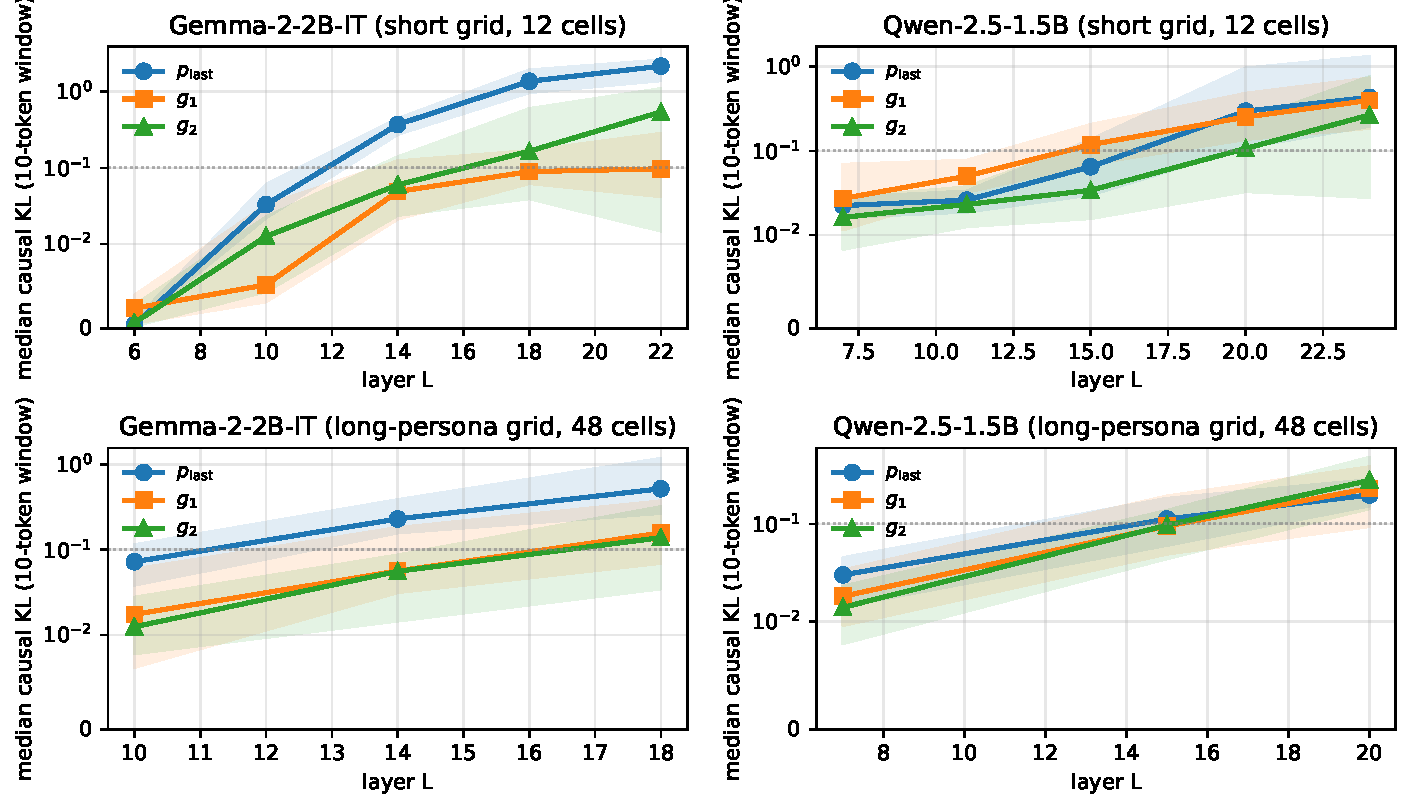
\includegraphics[width=\linewidth]{figures/localized_kl_by_layer.pdf}
\caption{Median causal KL under additive substitution at $p_{\text{last}}$ (blue), $g_1$ (orange), and $g_2$ (green), with 25th--75th percentile bands. Top row: 12-cell short grid on Gemma-2-2B-IT and Qwen-2.5-1.5B-Instruct. Bottom row: 48-cell long-persona grid on the same two models. Dotted gray line marks KL $=0.1$, a useful reference for ``essentially clean'' substitution. The localized additive regime is visible as an early/mid-layer band with low KL across all three positions, present on both models and on both grids.}
\label{fig:localized}
\end{figure}

\subsection{Interpretation}

The localized-position result changes the correct scope statement. The best-supported claim is no longer ``the additive approximation works at $p_{\text{last}}$,'' but:
\begin{quote}
\textbf{Persona-task composition is approximately additive in a localized residual-stream region near answer formation, spanning the last prompt position and the first generated-token positions.}
\end{quote}
This is materially stronger than a single-position claim, but still disciplined compared to a full-sequence mechanism.

\section{Robustness to Persona and Task Diversity}
\label{sec:diverse}

A result that holds only for a few personas and three tasks may still be fragile. We therefore test the same localized method on a much broader prompt grid.

\subsection{Long-persona grid}

On the 8-persona $\times$ 6-task grid (48 cells), we keep the probe positions fixed at $p_{\text{last}}$, $g_1$, and $g_2$, and evaluate a small early/mid/late layer set.

\paragraph{Gemma-2-2B-IT.}
The localized additive regime survives on the larger grid:
\begin{itemize}
    \item $p_{\text{last}}$: median KL $0.072$ at layer 10, $0.229$ at layer 14, $0.518$ at layer 18
    \item $g_1$: median KL $0.017$ at layer 10, $0.056$ at layer 14, $0.157$ at layer 18
    \item $g_2$: median KL $0.012$ at layer 10, $0.056$ at layer 14, $0.138$ at layer 18
\end{itemize}

The directional geometry also remains favorable. On Gemma-2-2B-IT at layer 14:
\begin{itemize}
    \item at $p_{\text{last}}$: median $\cos(\Delta_{XY}, \Delta_X + \Delta_Y)=0.818$
    \item at $g_1$: median $\cos(\Delta_{XY}, \Delta_X + \Delta_Y)=0.875$
\end{itemize}
At the same layers, median $\cos(\Delta_X,\Delta_Y)$ remains markedly smaller ($0.171$ at $p_{\text{last}}$, $0.234$ at $g_1$), so the additive story is not merely a trivial colinearity of all three vectors.

\paragraph{Qwen-1.5B-Instruct.}
The broader-grid result recurs cross-model:
\begin{itemize}
    \item $p_{\text{last}}$: median KL $0.030$ at layer 7, $0.112$ at layer 15, $0.198$ at layer 20
    \item $g_1$: median KL $0.018$ at layer 7, $0.095$ at layer 15, $0.231$ at layer 20
    \item $g_2$: median KL $0.014$ at layer 7, $0.097$ at layer 15, $0.279$ at layer 20
\end{itemize}
At Qwen layer 7, median $\cos(\Delta_{XY}, \Delta_X + \Delta_Y)$ is $0.862$ at $p_{\text{last}}$ and $0.936$ at $g_1$.

\begin{table}[t]
\centering
\small
\begin{tabular}{llccc}
\toprule
Model & Position & Early layer & Mid layer & Later layer \\
\midrule
Gemma-2-2B-IT & $p_{\text{last}}$ & L10: 0.072 [.038,.114] & L14: 0.229 [.157,.386] & L18: 0.518 [.266,1.17] \\
Gemma-2-2B-IT & $g_1$             & L10: 0.017 [.007,.059] & L14: 0.056 [.031,.182] & L18: 0.157 [.069,.374] \\
Gemma-2-2B-IT & $g_2$             & L10: 0.012 [.008,.028] & L14: 0.056 [.015,.087] & L18: 0.138 [.035,.320] \\
\midrule
Qwen-2.5-1.5B & $p_{\text{last}}$ & L7: 0.030 [.014,.045] & L15: 0.112 [.060,.183] & L20: 0.198 [.153,.284] \\
Qwen-2.5-1.5B & $g_1$             & L7: 0.018 [.010,.034] & L15: 0.095 [.049,.193] & L20: 0.231 [.094,.385] \\
Qwen-2.5-1.5B & $g_2$             & L7: 0.014 [.008,.023] & L15: 0.097 [.044,.137] & L20: 0.279 [.143,.481] \\
\bottomrule
\end{tabular}
\caption{Median causal KL on the 48-cell long-persona grid, with 25th--75th percentile range in brackets. The localized additive regime remains visible under substantially broader persona and task diversity.}
\label{tab:localized-diverse}
\end{table}

\subsection{Is the robustness broad-based or carried by a few easy cells?}

The larger-grid effect is not perfectly uniform, but it is broad-based enough for a paper claim. On Gemma-2-2B-IT at $p_{\text{last}}$, layer 14, per-persona median KLs range from roughly $0.14$--$0.39$ for most personas, with higher tails for a few outlier cells. On Qwen-1.5B-Instruct at $p_{\text{last}}$, layer 7, persona medians are tighter, mostly around $0.02$--$0.035$. Per-task medians on Gemma remain low-to-moderate across architecture review, planning, proposal review, policy commentary, haiku, and recommendation, rather than collapsing onto a single easy task family.

This is enough to support a careful robustness statement: the localized additive regime is not being carried by only one or two personas or tasks, though some tails remain and the result is not perfectly uniform at the cell level.

\section{Behavioral Verification of the Additive Substitution}
\label{sec:behavioral}

KL between teacher-forced distributions is a useful but indirect measure of whether the additive substitution preserves persona-conditioned behavior. A persona prompt should change \emph{what} the model talks about, not only the local probability of the next few tokens. We therefore complement the KL evidence in \cref{sec:localized,sec:diverse} with a behavioral-marker test that scores persona-specific output content directly, in the style of factual recall verification \cite{meng2022rome,todd2024function}.

\subsection{Protocol}

For each of the 8 long-form personas we define a small set of persona-specific surface markers chosen \emph{a priori} from the persona description itself. For example, the engineer persona is associated with markers including \texttt{SPOF}, \texttt{single point of failure}, \texttt{scalability}, \texttt{reliability}, \texttt{redundancy}; the counselor persona with markers including \texttt{feel heard}, \texttt{validate}, \texttt{compassion}; the doctor persona with \texttt{differential}, \texttt{symptoms}, \texttt{ruling out}. The full marker sets are listed in \cref{app:markers}. We hold out the marker selection from the experiment design --- markers are picked from the persona text, not from clean outputs.

For each (long persona, task) cell on the 8-persona $\times$ 3 review-task subset of the long-persona grid (24 cells), we generate 80 tokens greedily under four conditions:
\begin{itemize}
    \item \textbf{Clean}: \emph{``As [long persona], [task]''} with no intervention. This is the ceiling.
    \item \textbf{Additive}: same prompt, with $h_{BB} + \Delta_X + \Delta_Y$ substituted at $p_{\text{last}}$, layer~14.
    \item \textbf{Remove-X}: same prompt, with $h_{XY} - \Delta_X$ substituted at $p_{\text{last}}$, layer~14 (subtract the persona contribution).
    \item \textbf{Bare}: \emph{``[task]''} with no persona prefix and no intervention. This is the floor.
\end{itemize}

A cell scores \emph{any-marker} if at least one persona marker appears in the 80-token output (case-insensitive, word-boundary-aware). A faithful additive substitution should match the clean condition on this metric while remove-X and bare both drop substantially below it.

\subsection{Results}

\Cref{tab:markers} reports any-marker presence and average distinct-marker count under each condition.

\begin{table}[t]
\centering
\small
\begin{tabular}{lcc}
\toprule
Condition & Any persona marker present & Distinct markers (mean) \\
\midrule
Clean        & 16 / 24 (66.7\%) & 1.21 \\
Additive substitution at $p_{\text{last}}$, $L=14$ & 14 / 24 (58.3\%) & 0.92 \\
Remove-X at $p_{\text{last}}$, $L=14$ & 15 / 24 (62.5\%) & 0.96 \\
Bare prompt (no persona text)        & \phantom{0}1 / 24 (\phantom{0}4.2\%)  & 0.08 \\
\bottomrule
\end{tabular}
\caption{Behavioral-marker recovery on 8-persona $\times$ 3-task long-persona cells, scoring 80-token greedy continuations. ``Any'' columns count cells in which at least one persona marker appears; ``distinct'' columns count distinct markers per generation.}
\label{tab:markers}
\end{table}

Two findings stand out. First, the bare condition collapses to 4.2\% any-marker presence (1 of 24 cells), versus 66.7\% for clean. This is the strongest behavioral check we have that the persona text is doing real work in producing persona-conditioned output, and that the test detects when persona-specific content is absent. Second, the additive condition (58.3\%) tracks the clean ceiling (66.7\%) closely --- within roughly 13\% of clean and about 14$\times$ above the bare floor --- confirming that single-site additive substitution at $p_{\text{last}}$, $L=14$ does not degrade persona-conditioned output content. The distinct-marker column shows the same pattern in finer-grained form: clean at 1.21, additive at 0.92, bare at 0.08.

\subsection{Interpretation}

The clean--additive gap is small, and the clean--bare gap is large. That is the predicted shape for an additive substitution that preserves persona-conditioned behavior. The third row deserves separate comment: the remove-X intervention at $p_{\text{last}}$, $L=14$ (subtracting $\Delta_X$) does not substantially reduce marker presence (62.5\% vs.\ 66.7\% clean). This is consistent with the negative result in \cref{sec:no-replacement}: persona-conditioned content during multi-token generation flows in large part through attention back to the persona-text positions in the prompt, not through a single residual at $p_{\text{last}}$. Subtracting $\Delta_X$ at one site is too narrow to suppress persona behavior across the full 80-token continuation; only \emph{removing the persona text from the prompt entirely}, as in the bare condition, collapses persona-marker recovery.

The behavioral test therefore confirms two things in tandem: (i) the additive substitution preserves persona-conditioned output where the local additive picture is valid, and (ii) the persona contribution to multi-token generation is genuinely distributed, with single-site interventions insufficient to remove it. Both align with the picture developed in \cref{sec:no-replacement}: local additive structure is real and useful for predicting the next-step composition, but the wider mechanism producing persona-conditioned generation extends beyond the local additive region.

\section{What the Local Additive Story Does Not License}
\label{sec:no-replacement}

The most natural over-reading of the preceding sections is that a persona prompt can now be replaced by a vector. Our experiments do not support that claim.

\subsection{Host-prompt injection fails to replace persona text}

We tested a use-case-relevant setting based on long-form personas. The target prompt is a clean long-persona prompt; the host prompt is the corresponding baseline-persona prompt for the same task. We then substitute either:
\begin{itemize}
    \item the oracle clean residual $h_{XY}$ at $p_{\text{last}}$, or
    \item the cached additive prediction $h_{BB} + \Delta_X + \Delta_Y$ at $p_{\text{last}}$,
\end{itemize}
and compare 10-token KL against the clean long-persona continuation. For this experiment we use the 8-persona $\times$ 3 review-task subset of the long-persona grid (24 cells), matching the protocol of the original cache-and-inject experiments and keeping prompt structure consistent across cells.

Across these 24 long-persona cells, the host baseline median KL is $3.05$. Cached single-site substitution reduces this only slightly, to median KL $2.84$. Oracle substitution helps somewhat more (median KL $2.64$), but still falls well short of the clean target. This is the wrong outcome for a ``prompts are just vectors'' thesis.

\subsection{Wider multi-layer substitution does not fix the problem}

We also tried clamping the additive prediction at multiple layers simultaneously. On the same 24-cell setting:
\begin{itemize}
    \item single-layer substitution at layer 14: median KL $2.84$
    \item layers $\{10,12,14\}$: median KL $2.81$
    \item layers $\{10,12,14,16,18\}$: median KL $2.82$
    \item layers $\{10,12,14,16,18,20,22\}$: median KL $3.04$
    \item layers $\{6,8,10,12,14,16,18,20,22\}$: median KL $3.01$
\end{itemize}
The host baseline itself is $3.05$. Multi-layer clamping therefore does not materially close the host-to-target gap, and larger substitution windows begin to hurt.

\begin{table}[t]
\centering
\small
\begin{tabular}{lc}
\toprule
Condition & Median KL to clean long-persona target \\
\midrule
Host prompt, no substitution & 3.05 \\
Oracle single-site substitution at L14 & 2.64 \\
Cached additive substitution at L14 & 2.84 \\
Cached substitution at $\{10,12,14\}$ & 2.81 \\
Cached substitution at $\{10,12,14,16,18\}$ & 2.82 \\
Cached substitution at $\{10,12,14,16,18,20,22\}$ & 3.04 \\
Cached substitution at $\{6,8,10,12,14,16,18,20,22\}$ & 3.01 \\
\bottomrule
\end{tabular}
\caption{Long-persona host-prompt injection does not approach clean long-persona behavior. Better local additive prediction does not imply prompt replacement.}
\label{tab:host-inject}
\end{table}

\subsection{Interpretation}

This negative result is conceptually useful. The local additive story predicts next-step behavior in-context, but it does not replace the distributed information carried by persona text across prompt positions and the KV cache. During generation, later tokens continue to attend to the original prompt tokens. A single-site residual substitution can influence the next decision strongly without reproducing the full content of the original prompt state.

This gives a clean paper boundary:
\begin{quote}
\textbf{Local residual additivity near answer formation is real and useful, but it is not equivalent to full prompt compression or prompt replacement.}
\end{quote}

\section{Discussion}

The main strength of the current paper is not that it solves role prompting completely, but that it clarifies the right scale of claim.

The central result is strong precisely because it is scoped. The paper does not claim a full mechanism of role prompting. It claims that a localized additive regime exists near answer formation, that this regime survives broader prompt diversity, and that it has a sharp limit in the prompt-replacement setting.

First, the additive regime is localized but not isolated. It spans $p_{\text{last}}$, $g_1$, and $g_2$, which is exactly the region where a model is turning a prompt representation into the first few answer tokens. That is a more natural mechanistic object than a single hidden state at one prompt position.

Second, the result survives a broader and more realistic prompt grid. The use of long-form personas matters because modern role prompts are often descriptions rather than named entities. The use of six task families matters because recommendation, policy, review, planning, and constrained creative tasks pull on different output structures. The fact that the localized regime survives this broader grid makes the central claim much more credible.

Third, the negative host-injection result improves the paper rather than weakening it. It prevents a common over-interpretation and shows that the correct mechanistic picture has at least two levels: a localized additive regime near answer formation, and a wider distributed prompt/KV mechanism that local substitution does not erase.

Relative to prior work on activation steering and representation engineering \cite{turner2023actadd,zou2023representation}, the contribution here is not a new steering method, but a causal characterization of what kind of residual composition structure role prompts induce. Relative to ROME-style work \cite{meng2022rome}, we are not editing weights or claiming circuit-level closure. The paper sits at an intermediate level: higher than neuron ontology, lower than a full theory of prompt-conditioned computation.

\paragraph{Why the interaction term is not fatal to the additive story.}
The interaction term can be large in raw residual norm even when additive substitution remains causally strong. A useful framing is that the residual stream consumed by the next layer is post-normalization, not raw: a portion of the apparent magnitude gap between $h_{BB} + \Delta_X + \Delta_Y$ and $h_{XY}$ is absorbed by the next layer's RMSNorm before downstream computation sees it. We do not directly intervene on the normalization path here and so we report this only as a candidate explanation, not a mechanism. The operative observation for this paper is the empirical one: raw non-additivity in hidden-state norm does not by itself determine whether additive recomposition is behaviorally useful. The quantity that matters is downstream causal fidelity under substitution, and that fidelity is high in a localized region even when the interaction is not small in norm.

\paragraph{Why $(p_{\text{last}}, g_1, g_2)$ rather than a larger window.}
The probe positions are chosen to span the transition from prompt representation to the first answer tokens, which is the smallest object that captures \emph{both} the static prompt encoding and the model's online use of that encoding. Earlier positions inside the user turn can also show low-KL additive substitution, but their geometric statistics are less stable and their interpretation is less clean because they precede the model's prompt-to-answer transition. Later generated positions, beyond $g_2$, drift increasingly under teacher forcing and are not the natural mechanistic object for an online composition question.

\section{Limitations}

\begin{enumerate}
    \item \textbf{Localized, not full-sequence.} We study a small region near answer formation, not every prompt position or every generated token.
    \item \textbf{No circuit-level sufficiency.} The paper does not identify a minimal set of heads, neurons, or weights whose editing installs or removes a persona feature.
    \item \textbf{Prompt diversity is broader, not exhaustive.} The long-persona grid is much stronger than the short grid, but it is still English-only, cooperative, and single-turn.
    \item \textbf{Boundary cases remain.} Some late-layer and particular-cell tails are large. We have not systematically characterized which $(X,Y)$ combinations push the interaction term beyond the regime where additive substitution remains causally faithful.
    \item \textbf{Negative result is still local.} The failed prompt-replacement experiment shows that single-site substitution is insufficient, but it does not yet identify the correct distributed intervention.
    \item \textbf{Cross-model breadth is still selective.} The localized position result was checked across multiple model families, but the 48-cell robustness grid was only run on Gemma-2-2B-IT and Qwen-2.5-1.5B-Instruct.
\end{enumerate}

\section{Conclusion}

The cleanest statement supported by the current evidence is:

\begin{quote}
\textbf{In instruction-tuned language models, persona-task composition is approximately additive in a localized residual-stream region near answer formation, spanning the last prompt position and the first generated-token positions, but this local additive structure does not substitute for the distributed information carried by persona text in context.}
\end{quote}

This is narrower than a full mechanism of role prompting, but stronger than a single-position observation. It is supported by causal intervention, localized position extension, broader persona/task coverage, and cross-model recurrence. That is enough for a self-contained paper, and it leaves a clear next step for subsequent work: move from localized residual composition to distributed prompt/KV mechanisms.

\paragraph{Reproducibility.}
All experiments use HuggingFace \texttt{transformers} on a single Apple Silicon device with the \texttt{mps} backend. Gemma-2-2B-IT is loaded in \texttt{float32}; Qwen-2.5-1.5B-Instruct and Qwen-2.5-3B-Instruct are loaded in \texttt{bfloat16} (\texttt{float16} produces NaN residuals at the layers relevant here). Attention uses the \texttt{eager} implementation. All generation is greedy (\texttt{do\_sample=False}, \texttt{num\_beams=1}), so reported KLs and behavioral scores are deterministic functions of the model, prompt, and intervention. KL is computed by greedy 10-token continuation from the clean $XY$ prompt, followed by teacher-forced log-probability comparison across the same 10-token reference window under each intervention.

\paragraph{Code and artifacts.}
The main scripts supporting the paper are:
\begin{itemize}
    \item \texttt{scripts/v15\_localized\_positions.py} -- localized-position causal sweep (\cref{sec:localized})
    \item \texttt{scripts/v16\_diverse\_grid.py} -- broadened 8$\times$6 long-persona grid (\cref{sec:diverse})
    \item \texttt{scripts/v17\_behavioral\_markers.py} -- behavioral-marker recovery test (\cref{sec:behavioral})
    \item \texttt{scripts/v14b\_v2\_inject.py} -- host-prompt single-site substitution (\cref{sec:no-replacement})
    \item \texttt{scripts/v14e\_multilayer\_inject.py} -- multi-layer substitution (\cref{sec:no-replacement})
\end{itemize}

\appendix

\section{Prompt Grids}

\subsection{Original short grid}

\paragraph{Personas.}
The short-grid persona set is:
\begin{itemize}
    \item Warren Buffett
    \item Karl Marx
    \item Yoda
    \item Maya Angelou
\end{itemize}

\paragraph{Tasks.}
The short-grid task set is:
\begin{itemize}
    \item ``Comment on whether universal basic income is a good policy.''
    \item ``Write a haiku about Monday mornings.''
    \item ``Recommend a book worth reading and explain why.''
\end{itemize}

\paragraph{Baselines.}
The baseline persona is ``a thoughtful person'' and the baseline task is ``Give advice to someone facing a difficult decision.''

\subsection{Broadened long-persona grid}

\paragraph{Personas.}
The long-persona set is:
\begin{itemize}
    \item a senior software engineer with 10 years of experience who pays close attention to architecture, reliability, and avoiding single points of failure
    \item an empathetic counselor with deep training in active listening, cognitive behavioral therapy, and trauma-informed care, who helps clients feel heard without imposing solutions
    \item a pragmatic startup founder who has bootstrapped three companies, makes capital-efficient decisions, iterates fast based on user feedback, and avoids vanity metrics
    \item a middle school science teacher who has taught for 15 years, explains concepts with relatable analogies, gently checks for understanding, and meets students at their level
    \item an investigative journalist who has covered city government for two decades, asks pointed questions, follows the money, and verifies every claim against primary sources
    \item a primary-care physician who has practiced for 25 years, listens carefully to symptoms, considers differential diagnoses without alarming the patient, and explains options clearly
    \item a corporate litigator who has tried cases at the appellate level for 20 years, anticipates opposing arguments, builds case theory from the record, and communicates dense law in plain English
    \item a head chef trained in classical French technique who has run three Michelin-starred kitchens, builds menus around seasonal ingredients, and teaches young cooks by demonstration
\end{itemize}

\paragraph{Tasks.}
The long-persona task set is:
\begin{itemize}
    \item architecture review: ``Review this design: a microservice architecture where eight services share a single PostgreSQL database for both transactional state and event log.''
    \item startup-plan review: ``Review this plan: a three-person team building a B2B SaaS product, planning to launch in three months, with no usage analytics in v1.''
    \item scheduling-proposal review: ``Review this proposal: an internal tool that automates calendar scheduling using an LLM, sending tentative meetings to all parties before confirmation.''
    \item policy commentary: ``Comment on whether universal basic income is a good policy.''
    \item constrained creative: ``Write a haiku about Monday mornings.''
    \item recommendation: ``Recommend a book worth reading and explain why.''
\end{itemize}

\section{Behavioral Markers}
\label{app:markers}

The persona marker sets used in \cref{sec:behavioral}. Markers were selected from each persona's description before running the experiment.

\begin{itemize}
\item \textbf{engineer}: \texttt{SPOF}, \texttt{single point of failure}, \texttt{scalability}, \texttt{scalable}, \texttt{reliability}, \texttt{fault tolerance}, \texttt{fault-tolerant}, \texttt{redundancy}, \texttt{resilience}, \texttt{throughput}, \texttt{latency}, \texttt{consistency}, \texttt{availability}.
\item \textbf{counselor}: \texttt{feel heard}, \texttt{validate}, \texttt{validated}, \texttt{acknowledge}, \texttt{acknowledged}, \texttt{your experience}, \texttt{your feelings}, \texttt{compassion}, \texttt{compassionate}, \texttt{without judgment}, \texttt{trauma-informed}, \texttt{active listening}, \texttt{feelings}, \texttt{emotion}.
\item \textbf{founder}: \texttt{iterate}, \texttt{iterating}, \texttt{iteration}, \texttt{MVP}, \texttt{minimum viable}, \texttt{user feedback}, \texttt{customer feedback}, \texttt{capital-efficient}, \texttt{lean}, \texttt{runway}, \texttt{validation}, \texttt{ship}, \texttt{shipping}, \texttt{product-market fit}, \texttt{vanity metric}, \texttt{traction}, \texttt{burn}, \texttt{bootstrapped}.
\item \textbf{teacher}: \texttt{imagine}, \texttt{think of}, \texttt{like a}, \texttt{analogy}, \texttt{analogies}, \texttt{for example}, \texttt{step by step}, \texttt{step-by-step}, \texttt{students}, \texttt{understand}, \texttt{let's say}, \texttt{picture this}, \texttt{as if}.
\item \textbf{journalist}: \texttt{sources}, \texttt{source}, \texttt{primary source}, \texttt{primary sources}, \texttt{follow the money}, \texttt{accountability}, \texttt{transparency}, \texttt{investigate}, \texttt{verify}, \texttt{verified}, \texttt{on the record}, \texttt{off the record}, \texttt{evidence}, \texttt{public interest}, \texttt{pointed question}, \texttt{track record}.
\item \textbf{doctor}: \texttt{symptom}, \texttt{symptoms}, \texttt{diagnosis}, \texttt{diagnose}, \texttt{differential}, \texttt{patient}, \texttt{treatment}, \texttt{ruling out}, \texttt{rule out}, \texttt{clinical}, \texttt{examination}, \texttt{condition}, \texttt{medication}, \texttt{evaluate}, \texttt{underlying}, \texttt{comorbid}.
\item \textbf{lawyer}: \texttt{liability}, \texttt{liabilities}, \texttt{jurisdiction}, \texttt{statute}, \texttt{precedent}, \texttt{evidence}, \texttt{evidentiary}, \texttt{opposing}, \texttt{counterparty}, \texttt{due diligence}, \texttt{parties}, \texttt{indemnif*}, \texttt{contractual}, \texttt{compliance}, \texttt{compliant}, \texttt{jurisprudence}, \texttt{case theory}, \texttt{on the record}.
\item \textbf{chef}: \texttt{seasonal}, \texttt{season}, \texttt{ingredient}, \texttt{ingredients}, \texttt{flavor}, \texttt{flavour}, \texttt{palate}, \texttt{fresh}, \texttt{simmer}, \texttt{saut\'e}, \texttt{saute}, \texttt{balance}, \texttt{garnish}, \texttt{mise en place}, \texttt{technique}, \texttt{classical}, \texttt{French}.
\end{itemize}

\section{Artifact Map}

The key result files used in the paper are:
\begin{itemize}
    \item \texttt{results/v15\_gemma2b\_localized\_positions.json}
    \item \texttt{results/v15\_qwen15\_localized\_positions.json}
    \item \texttt{results/v15\_qwen3b\_localized\_positions.json}
    \item \texttt{results/v16\_gemma2b\_diverse\_grid.json}
    \item \texttt{results/v16\_qwen15\_diverse\_grid.json}
    \item \texttt{results/v17\_behavioral\_markers.json}
    \item \texttt{results/v14b\_v2.json}
    \item \texttt{results/v14e\_multilayer.json}
\end{itemize}

\bibliographystyle{plain}
\bibliography{refs}

\end{document}
